% Value-equal strict errors of the OOF writers (Sec. 7, Table 14 of the paper).
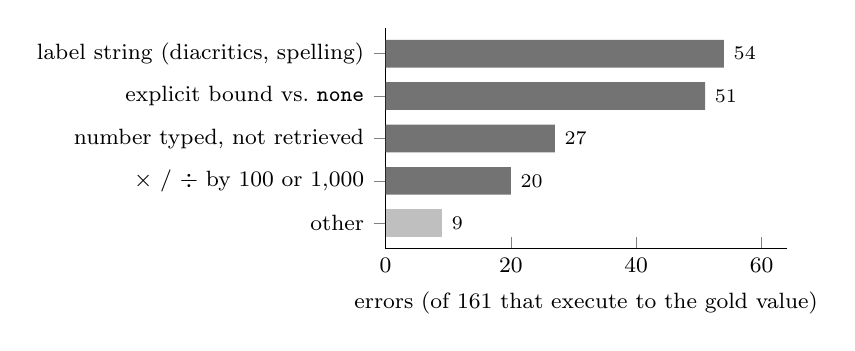
\begin{tikzpicture}
  \begin{axis}[
      width=0.42\linewidth, height=2.8cm, scale only axis,
      xbar, bar width=10pt, bar shift=0pt,
      xmin=0, xmax=64,
      ytick={1,...,5}, y dir=reverse,
      yticklabels={{label string (diacritics, spelling)},{explicit bound vs.\ \texttt{none}},{number typed, not retrieved},{$\times$ / $\div$ by 100 or 1,000},{other}},
      yticklabel style={font=\footnotesize, align=right},
      enlarge y limits=0.15,
      xlabel={errors (of 161 that execute to the gold value)},
      xlabel style={font=\footnotesize},
      tick label style={font=\footnotesize},
      axis x line*=bottom, axis y line*=left,
      nodes near coords, nodes near coords style={font=\scriptsize\bfseries},
    ]
    \addplot[fill=black!55, draw=none] coordinates {(54,1) (51,2) (27,3) (20,4)};
    \addplot[fill=black!25, draw=none] coordinates {(9,5)};
  \end{axis}
\end{tikzpicture}
